% --------------------------------------------------------------------------- %
% --------------------------------------------------------------------------- %
\section{The Large Hadron Collider}
\label{sec:lhc}

The Large Hadron Collider (LHC) is the world's largest and most powerful particle accelerator ever constructed \cite{Evans:2008zzb}. The accelerator was constructed and is operated by the European Organization for Nuclear Research (CERN), and straddles the border between Switzerland and France near Geneva. The accelerator tunnels of the LHC are 27 kilometers in circumferences and 50-175 meters underground, as well as additional, smaller rings used to accelerate protons before they are injected into the LHC. An aerial view of the LHC layout and location of the different experiments is shown in figure \ref{fig:lhcAerial}.

\begin{figure}
	\centering
	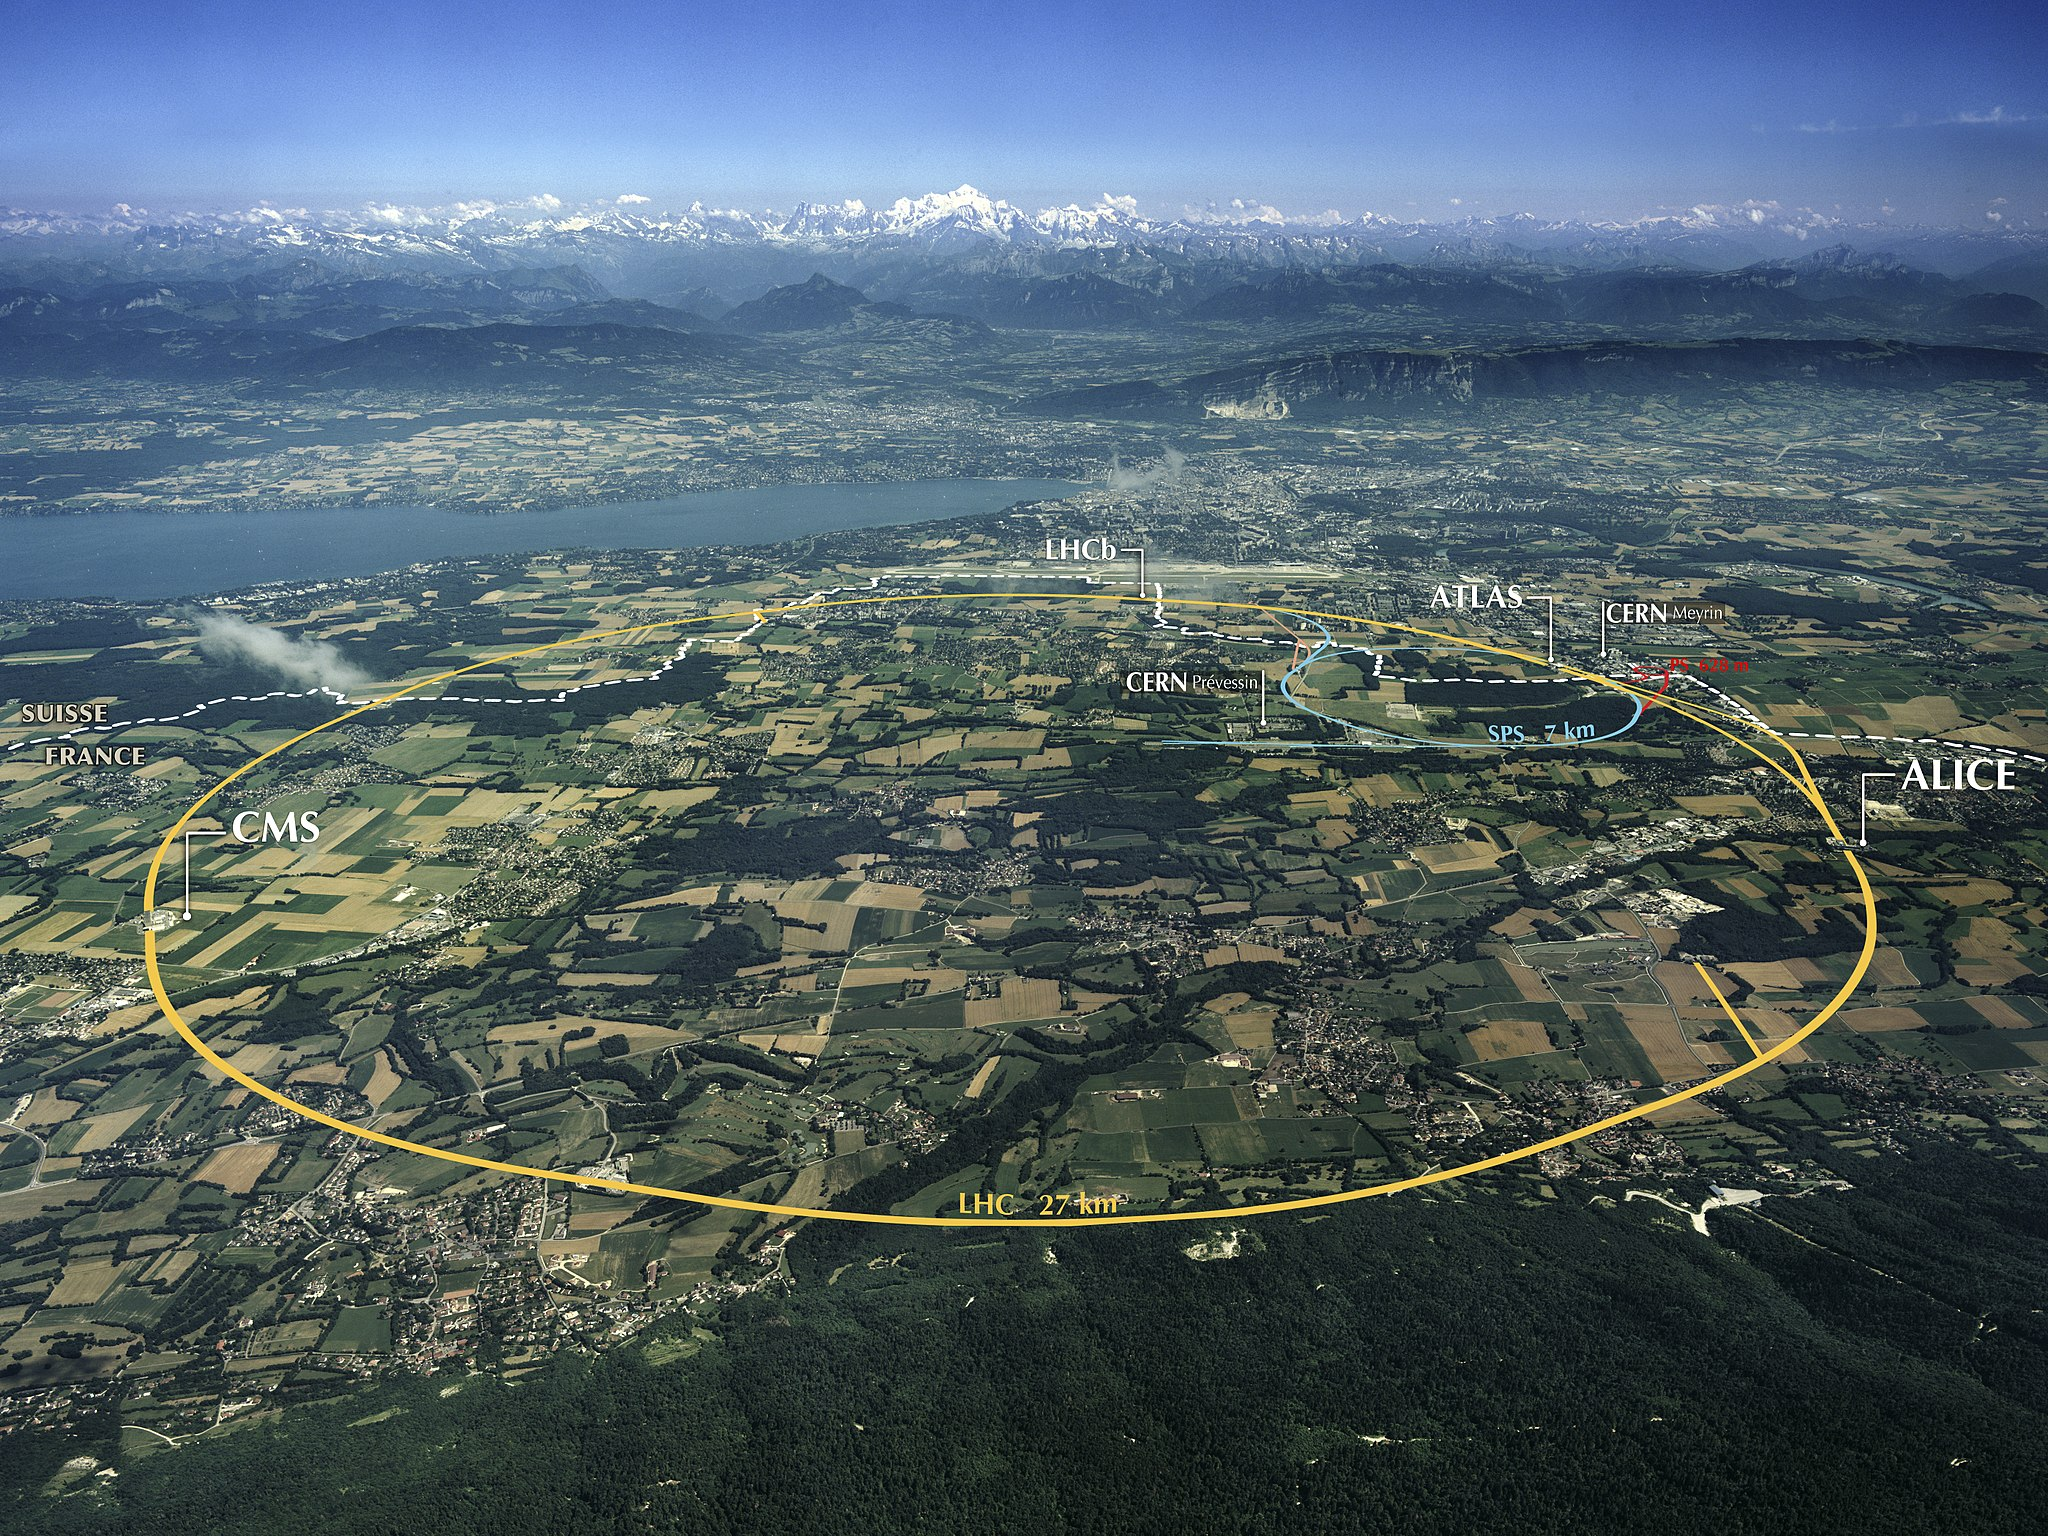
\includegraphics[width=0.95\textwidth]{detector/figs/2048px-CERN_Aerial_View.jpg}
	\renewcommand{\baselinestretch}{1.0}
	\caption[An aerial view of CERN and the LHC complex.]{An aerial view of CERN and the LHC complex. The colored lines indicate the location of the underground tunnels of the LHC and other booster rings used to accelerate protons. \cite{cc}}
	\label{fig:lhcAerial}
\end{figure}

The protons delivered by the LHC are accelerated in stages before reaching final collision energy. First, protons are accelerated to 50\MeV by a linear accelerator before being injected into the Proton Synchrotron Booster (PSB). The PSB accelerates protons to 1.4\GeV before they are injected into the Proton Synchrotron (PS) and accelerated to 26\GeV, then injected into the Super Proton Synchrotron (PSP) and accelerated to 450\GeV. Finally the protons are injected into the LHC and directed in two parallel beamlines in opposite directions to a beam energy of 6.5\TeV. A schematic representation of the different boost rings is illustrated in figure \ref{fig:lhcSchematic}. 

\begin{figure}
	\centering
	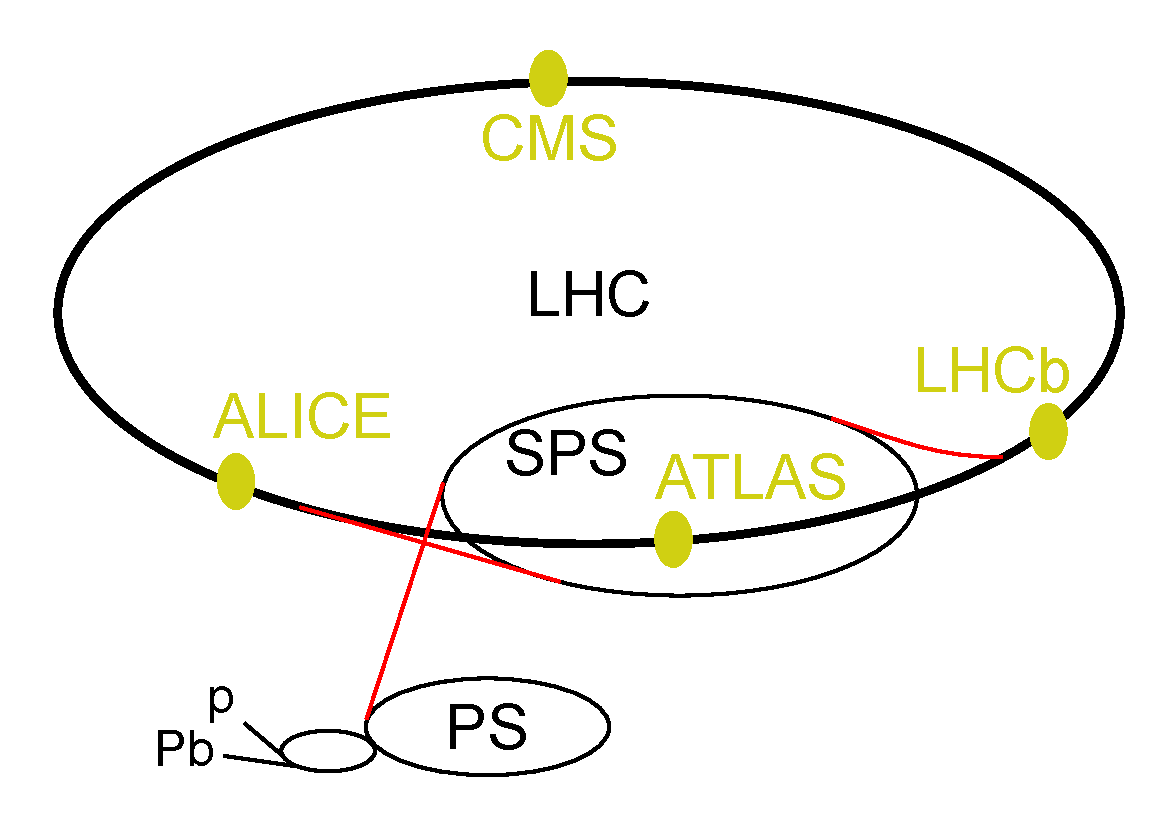
\includegraphics[width=0.75\textwidth]{detector/figs/LHC}
	\renewcommand{\baselinestretch}{1.0}
	\caption[A schematic of the different accelerator rings used by the LHC.]{A schematic of the different accelerator rings used by the LHC. Protons are accelerated in a series of booster rings -- the Proton Synchrotron Booster (PSB, not labeled), Proton Synchrotron (PS), and Super Proton Synchrotron (SPS) -- before they are injected into the LHC and ramped up to their collision energy. Particles can be directed to collide at any of the interaction points along the ring where different detectors are situated. \cite{cc}}
	\label{fig:lhcSchematic}
\end{figure}

The total amount of proton-proton collisions delivered by the LHC is often measured by the {\it integrated luminosity}. The {\it instantaneous luminosity} (L) is a measure of the number of interactions that can be produced per unit area per second, and the integrated luminosity ($\mathcal{L}$) is the total luminosity integrated over some time interval. Integrated luminosity is thus a unit of inverse area and typically measured in barns (1 barn = 100 $\text{fm}^2$). The total number of a particular type of event measured by a detector $N_{\mathrm{events}}$ is the product of the integrated luminosity, the cross section for that particular process ($\sigma$), and the detector-determined efficiency ($\epsilon$) as described in equation \ref{eq:lumi}. The total integrated luminosty delivered by the LHC compared that recorded by CMS is illustrated in figure \ref{fig:lumi}.
\begin{equation}
	N_{\mathrm{events}} = \mathcal{L} \cdot \sigma \cdot \epsilon
	\label{eq:lumi}
\end{equation}

\begin{figure}
	\centering
	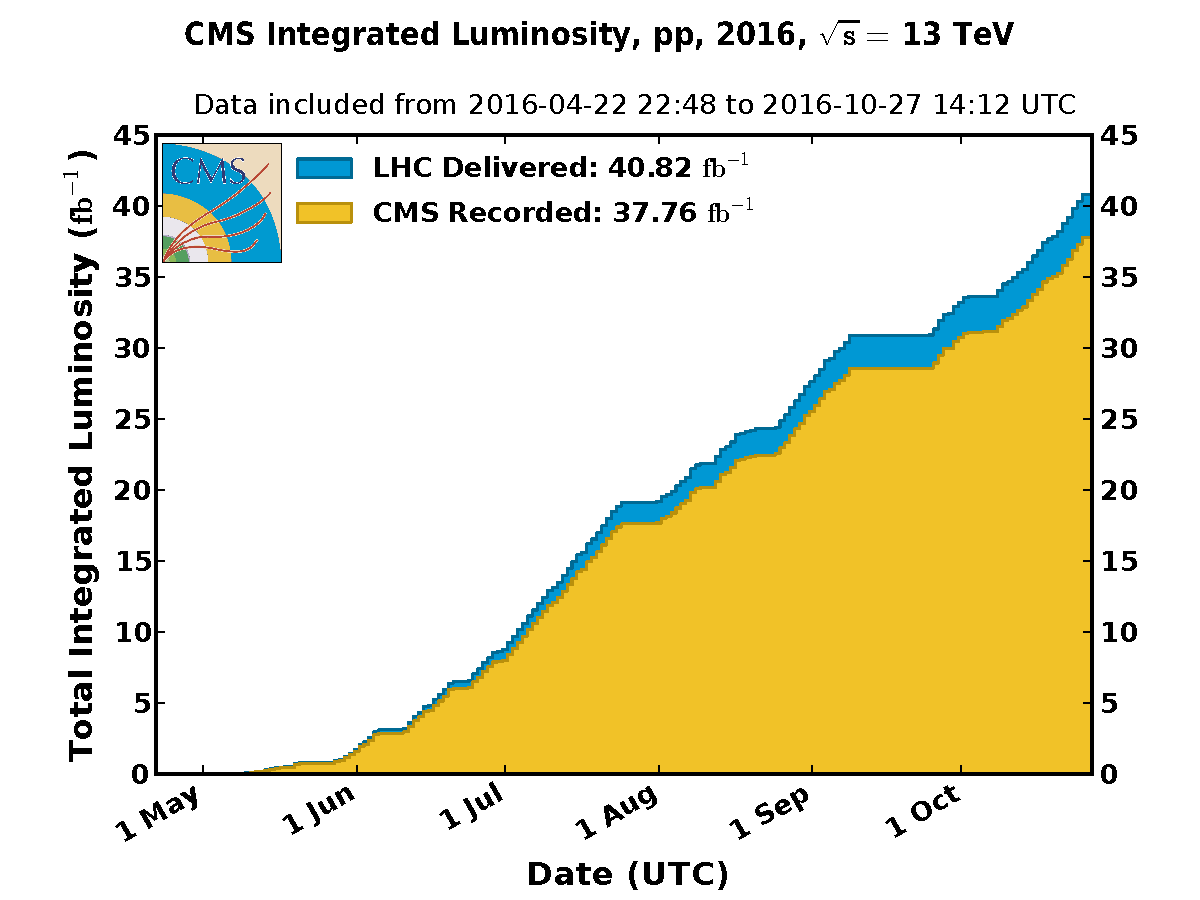
\includegraphics[width=0.95\textwidth]{detector/figs/int_lumi_per_day_cumulative_pp_2016}
	\renewcommand{\baselinestretch}{1.0}
	\caption[The total integrated luminosity delivered by the LHC at a center-of-mass energy of 13\TeV compared to that recorded by CMS through 2016.]{The total integrated luminosity delivered by the LHC at a center-of-mass energy of 13\TeV compared to that recorded by CMS through 2016.}
	\label{fig:lumi}
\end{figure}

\subsection{Proton Bunches and Pileup}
\label{subsec:pileup}

The protons delivered by the LHC are not in a continuous stream, but separated into ``bunches'' so that interactions occur at discrete intervals. Each proton bunch is approximately 30 centimeters long and contains over 100 billion protons at the beginning of the machine fill. Proton bunches are injected into the LHC and stored with a bunch spacing of 25ns (or 40 MHz), where they can be accelerated and for hours while collisions occur at the interaction points.

Because protons are delivered in discrete bunches at such a high rate, any bunch crossing results in multiple interactions and outgoing products. This is known as {\it pileup}, and presents a significant challenge for physics detectors which must be able to associate outgoing products to a specific interaction. {\it In-time pileup} is caused by multiple interactions per bunch crossing (the majority of interaction in a given bunch crossing are soft proton-proton inelastic scattering), and {\it out-of-time pileup} is due to interactions from a different bunch crossing (such as the read-out time of a detector subsystem). An effective detector needs to correctly identify which particles are associated with the interaction of interest in any given event, and mitigate the effects of pileup in design and construction.

% --------------------------------------------------------------------------- %
% --------------------------------------------------------------------------- %
